% -*-coding: utf-8 -*-
% Держать в начале каждого файла!

\documentclass[a4paper, 12pt]{extarticle}
\usepackage{metod}

\MTDSetPhysSection{Механика}
\MTDSetTitle{Определение модуля Юнга методом тензометрии}
\MTDDesignator{М--9A}
\MTDSetGrade{10}

\MTDSetAuthors{И.~Н.~Грачева, В.~И.~Гребенкин, А.~Е.~Иванов, И.~А.~Коротова,
Е.~И.~Красавина, А.~В.~Кравцов, Н.~С.~Кулеба, Б.~В.~Падалкин,
Г.~Ю.~Шевцова, Т.~С.~Цвецинская}

\MTDSetEditorsGenCase{И.~Н.~Грачевой, А.~Е.~Иванова, А.~В.~Кравцова}

\newcommand{\eps}{\epsilon}

\begin{document}

\MTDTitlePage
\MTDInfoPage

\setcounter{section}{9}

\subsection{Цель работы}
Целью работы является экспериментальное определение модуля Юнга методом тензометрии и знакомство с этим методом. 

\subsection{Основные теоретические сведения о методе тензометрии}
Между силой, растягивающей металлический стержень, и его удлинением существует линейная зависимость. Она носит название закона Гука, и записывается обычно в виде 
\begin{equation}
\label{eq:m9a-hooke's-law}
\sigma = E \eps,
\end{equation}
где $\sigma$ "--- \emph{механическое напряжение} в стержне, определяющееся по формуле:
\begin{equation}
\label{eq:m9a-strain}
\sigma = \frac{F}{A}, %;
\end{equation}
%нужно ли "где"
$F$ "--- растягивающая сила, $A$ "--- площадь поперечного сечения стержня; $\eps$  "--- \emph{относительная деформация} стержня, которая выражается формулой:
\begin{equation}
\label{eq:m9a-relative-strain}
\eps = \frac{\Delta L}{L},
\end{equation}
$\Delta L$ "--- приращение длины стержня, $L$ "--- его первоначальная длина; $E$ "--- коэффициент пропорциональности, называемый \emph{модулем Юнга}. 

\textbf{Примечание.} Закон Гука справедлив не всегда. При усилиях, больших некоторого порогового значения, называемого пределом текучести, связь между напряжением и деформацией становиться нелинейной, а затем растянутый стержень разрушается. В пределах упругости, то есть когда действует закон Гука, металлы деформируются очень мало,  длина растянутого стержня возрастает не более чем на 0,01--0,05\% от первоначального размера. Размеры машин и приборов рассчитывают так, чтобы действующие на них нагрузки не приводили к появлению напряжений, превышающих предел текучести. Для оценки правильности расчетов на прочность очень важно знать, какие напряжения и деформации в действительности возникают в конструкции при действии нагрузки. Для этого, как правило, измеряют деформации и по ним вычисляют напряжения. 

\begin{figure}[h]
\centering
\begin{minipage}[b]{0.45\linewidth}
\centering
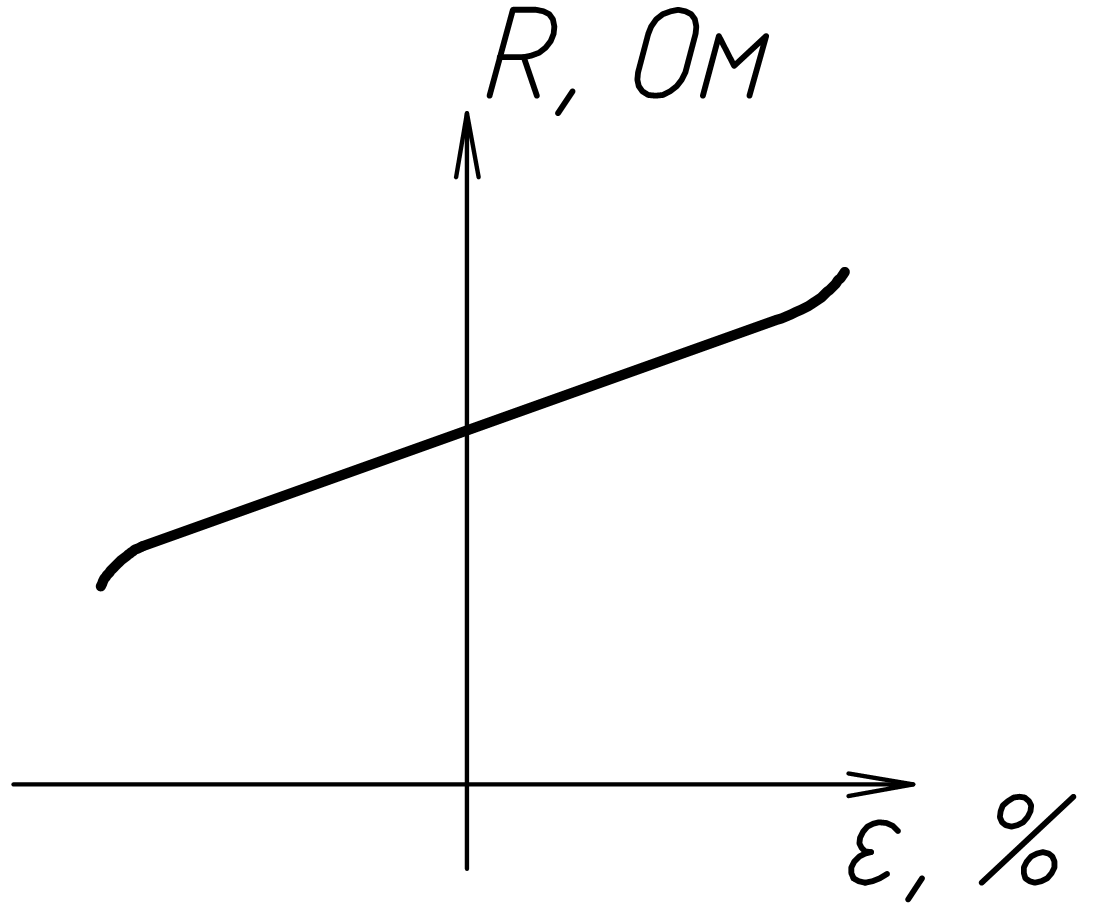
\includegraphics[width=0.7\linewidth, keepaspectratio=true]{M9-PressureSensorGraph}
\caption{\label{fig:m9a-resistance}}
\end{minipage} \hfill
\begin{minipage}[b]{0.45\linewidth}
\centering
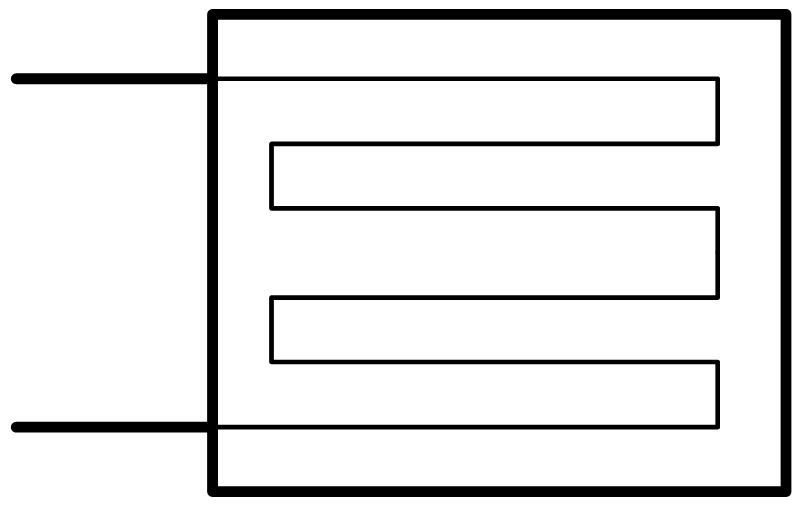
\includegraphics[width=0.7\linewidth, keepaspectratio=true]{M9-PressureSensor}
\caption{\label{fig:m9a-resistive-strain-sensor}}
\end{minipage}
\end{figure}

Для измерения деформаций используется свойство некоторых материалов изменять удельное электрическое сопротивление в зависимости от деформации. Например, у константана "--- сплава, состоящего из 60\% меди и 40\% никеля, электрическое сопротивление в определенных пределах линейно зависит от деформации (рис.~\ref{fig:m9a-resistance}). Это свойство использовано для создания \emph{тензорезисторов} "--- датчиков для измерения деформации. Тензорезистор (рис.~\ref{fig:m9a-resistive-strain-sensor}) представляет собой решетку из проволоки или фольги, наклеенной на непроводящую основу, и выводных проводников. %ИЗМ: запятая после "основу"

Тензорезистор наклеивают на поверхность металла и в качестве активного сопротивления включают в цепь. Для определения величины и знака деформации часто используется мостовая схема, изображенная на рис.~\ref{fig:m9a-scheme}. Тензорезистор, предназначенный для измерения деформации, включается в одно из плеч моста как сопротивление $R_1$. На клеммы цепи $AB$ подается постоянное напряжение, а между точками $C$ и $D$ подключается гальванометр. Между сопротивлениями $R_3$ и $R_4$ находится переменное сопротивление "--- реохорд. Его ползунок электрически соединен с гальванометром, и при перемещении ползунка сопротивление плеч меняется. Мост сбалансирован, если:
\begin{equation}
\label{eq:m9a-resistance}
R_1 R_3 = R_2 R_4.
\end{equation}
При этом разность потенциалов между точками $C$ и $D$ равна нулю. Когда тензорезистор под действием нагрузки изменяет свое сопротивление, между точками $C$ и $D$ возникает разность потенциалов. Как правило, применяют \emph{нулевой метод} измерения, при котором мост сбалансируется вновь путем изменения сопротивлений $R_3$ и $R_4$ с помощью реохорда. Величина смещения ползунка реохорда и определяет меру деформации. Признаком того, что мост сбалансирован, служит нулевое показание гальванометра.

Сопротивление $R_2$ тоже представляет собой тензорезистор, который размещают вблизи от активного тензорезистора $R_1$. Изменение температуры приводит к одинаковому изменению их сопротивлений, и баланс моста не нарушается. Поэтому сопротивление $R_2$ называют температурным компенсатором (или компенсирующим тензорезистором).

Обычно сопротивления $R_3$ и $R_4$, гальванометр, блок питания и реохорд объединяются в один прибор "--- измеритель деформации. К нему подключаются активный тензорезистор $R_1$ и температурный компенсатор $R_2$. 

\begin{figure}[h]
\begin{center}
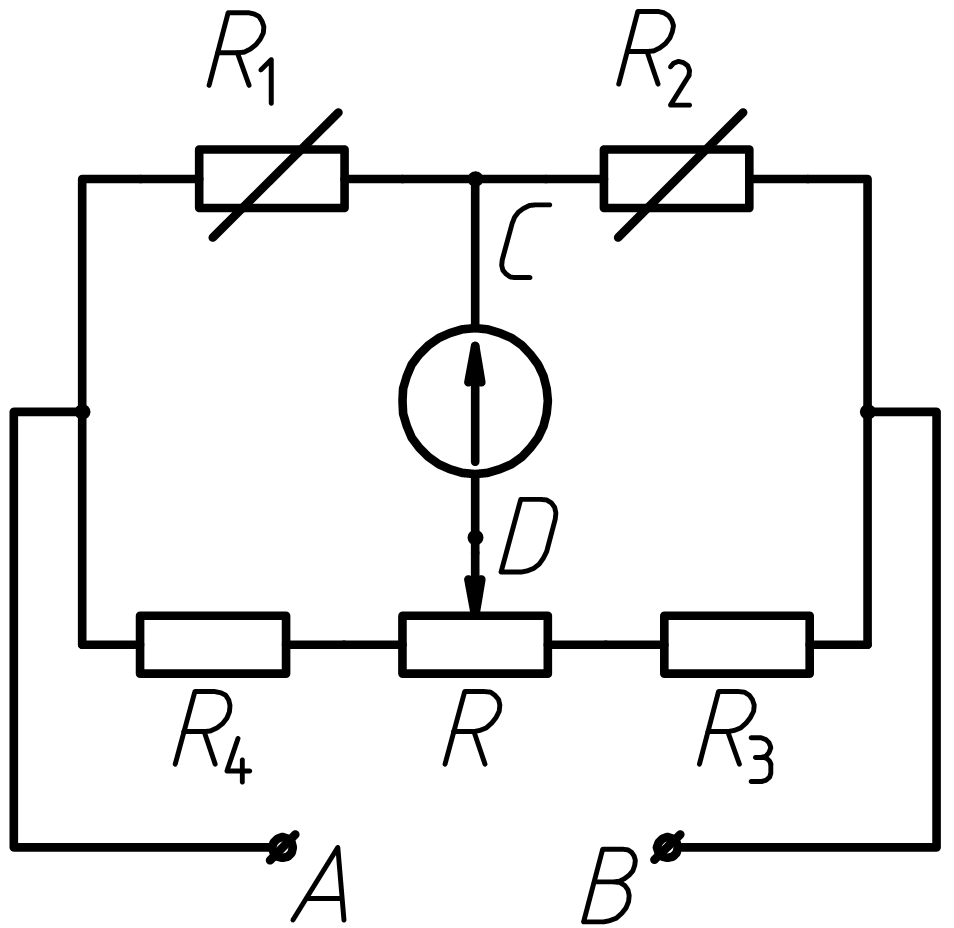
\includegraphics[width=0.37\linewidth, keepaspectratio=true]{M9-WheatstoneBridgeSchematic}
\end{center}
\caption{\label{fig:m9a-scheme}}
\end{figure}
%возможно, она слишком большая и надо делать wrapfigure. тут есть дилемма: либо сделать так, чтобы след. параграф был на след. странице, либо сделать так, чтобы контрольный вопрос не повис на одной странице; странное противоречивое описание реохорда в тексте 

\subsection{Методика выполнения работы и описание экспериментальной установки}
В лабораторной работе используется алюминиевый стержень. Он установлен в деревянной раме (рис.~\ref{fig:m9a-equipment}). Растягивающая сила создается рычагом, короткое плечо которого соединено со стержнем, а на длинное подвешиваются грузы. Соотношение плеч составляет $1:8$. Активный тензорезистор, предназначенный для измерения деформации стержня, наклеен на него в центре. Компенсирующий тензорезистор наклеен на алюминиевую площадку на рычаге. Выводные проводники обоих тензорезисторов закрыты, чтобы избежать повреждений. Тензорезисторы подключаются к электронному измерителю деформации. 

Цель работы "--- экспериментальное определение модуля Юнга алюминия. Для этого алюминиевый стержень растягивается заранее заданной силой, его деформация измеряется с помощью тензорезистора, и из закона Гука~\eqref{eq:m9a-hooke's-law} вычисляется модуль Юнга: 
\begin{equation}
\label{eq:m9a-young's-modulus}
E = \frac{\Delta \sigma}{\Delta \eps} = \frac{\Delta F / A}{K_\eps \Delta N},
\end{equation}
где $\Delta \sigma$ "--- приращение напряжения, $\Delta \eps$ "--- приращение деформации, $\Delta F$ "--- приращение растягивающего усилия, $\Delta N$  "--- приращение показаний измерителя деформации, $K_\eps$ "--- цена деления измерителя деформации. 

\begin{figure}[h]
\begin{center}
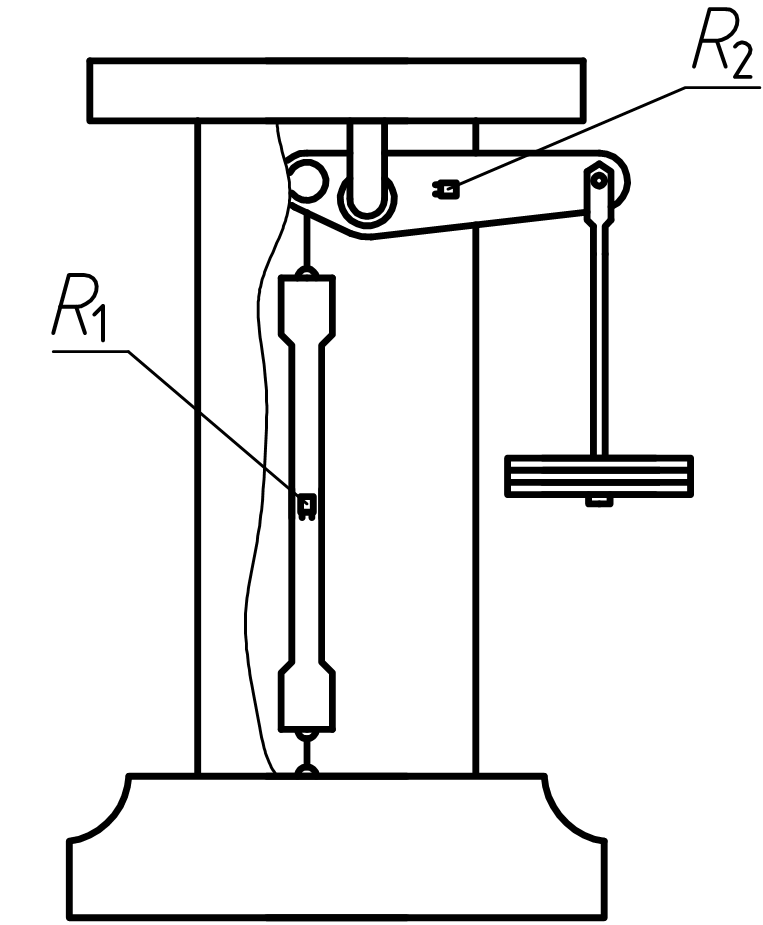
\includegraphics[width=0.4\linewidth, keepaspectratio=true]{M9-StrainGaugePlacement}
\end{center}
\caption{Схема размещения терморезисторов\label{fig:m9a-equipment}}
\end{figure}


\subsection{Порядок выполнения работы}

\begin{table}[h]
\caption{\label{tab:m9a-res-exp}}
\begin{flushright}
\begin{tabular}{|c|c|c|c|c|}
\hline
\multirow{4}*{\textnumero} & \multirow{4}{1.7cm}{\centering Масса груза, кг} & \multirow{4}{3.0cm}{\centering Растягивающая сила $F,~\Units{\text{Н}}$} & \multirow{4}{4.7cm}{\centering Показания измерителя деформации $N$, \Units{делений шкалы}} &  \multirow{4}{4.8cm}{\centering Приращение показания измерителя деформации, делений шкалы} \\
& & & & \\
& & & & \\
& & & & \\ \hline
1 & --- & --- & & ---  \\ \hline
2 & 1 & & & \\ \hline
3 & 2 & & & \\ \hline
4 & 3 & & & \\ \hline
5 & 4 & & & \\ \hline
6 & 5 & & & \\ \hline
\end{tabular}
\end{flushright}
\end{table}

\begin{enumerate}
\item Проверьте правильность присоединения проводов к электронному измерителю деформаций. 
\item Включите питание электронного измерителя, переведя переключатель в положение <<Работа>>. 
\item Сбалансируйте мост, вращая рукоятку реохорда. Стрелка гальванометра должна быть на отметке <<0>>. Запишите в таблицу~\ref{tab:m9a-res-exp} показания измерителя деформации.
\item Подвесьте на рычаг груз массой 1~\Units{кг}, вновь сбалансируйте мост и запишите новое показание измерителя. 
\item Добавляя грузы, доведите общую нагрузку до 5~\Units{кг}. После каждого увеличения нагрузки вновь сбалансируйте мост и запишите показания измерителя. 
\item Снимите все грузы, сбалансируйте мост и отключите питание электронного измерителя. 
\item Подсчитайте растягивающую силу и приращения показаний измерителя деформации, соответствующие одной ступени нагружения. Постройте график зависимости $F(N)$. 
\item Подсчитайте среднее приращение показаний измерителя деформации на одной ступени нагружения. Определите модуль Юнга.

Среднее приращение показаний измерителя деформации (в делениях шкалы) рассчитайте по формуле:
\[
\overline{\Delta N} = \frac{\Delta N_1 + \Delta N_2 + \Delta N_3 + \Delta N_4 + \Delta N_5}{5} %о, другое среднее... изменить на MTDMean?
\]

Модуль Юнга можно вычислить по формуле~\eqref{eq:m9a-young's-modulus}. \\
Для расчетов используйте следующие данные: размеры поперечного сечения стержня: $2,5~\Units{\text{мм}} \times 14~\Units{\text{мм}}$, площадь его поперечного сечения $A = 35~\Units{\text{мм}^2}$; цена деления измерителя деформации $K_\eps = 7,2 \cdot 10^{-8}~\Units{\text{единиц деформации} / \text{деление шкалы}}$. 
\end{enumerate}

\subsection{Контрольные вопросы}
\begin{enumerate}
\item Сформулируйте закон Гука, запишите его аналитическое выражение и укажите единицы входящих в него физических величин. 
\item Что называется механическим напряжением?
\item Что такое модуль упругости (модуль Юнга)? Какова единица СИ модуля упругости?
\item Как связаны коэффициент жесткости и модуль Юнга?
\item Если пружину жесткости~$k$ разрезать пополам, то какой будет жесткость каждой половинки пружины? 
\item Если однородный цилиндрический стержень подвесить за один конец к потолку, то каким будет удлинение~$\Delta L$ стержня под действием его собственного веса? Длина стержня равна~$L$. Считайте, что плотность материала стержня~$\rho$ и его модуль Юнга~$E$ известны. 
\end{enumerate}

\end{document}
